\documentclass{sig-alternate-10}
\usepackage{tikz}
\usetikzlibrary{arrows,positioning}
\def\sharedaffiliation{\end{tabular}\newline\begin{tabular}{c}}
\newtheorem{example}{Example}[section]
\newcommand{\keyword}[1]{\textup{\textsf{#1}}}
\newcommand{\Dept}{\keyword{Dept}}
\newcommand{\Emp}{\keyword{Emp}}
\newcommand{\Text}{\keyword{Text}}
\newcommand{\Int}{\keyword{Int}}
\newcommand{\Department}{\keyword{department}}
\newcommand{\Employee}{\keyword{employee}}
\newcommand{\Name}{\keyword{name}}
\newcommand{\Position}{\keyword{position}}
\newcommand{\Salary}{\keyword{salary}}
\newcommand{\Manager}{\keyword{manager}}
\newcommand{\Subordinate}{\keyword{subordinate}}

\begin{document}

\title{Query Combinators}

\numberofauthors{2}
\author{
    \alignauthor Clark C. Evans \\ \email{cce@clarkevans.com}
    \alignauthor Kyrylo Simonov \\ \email{xi@resolvent.net}
    \sharedaffiliation
    \affaddr{Prometheus Research, LLC} \\
}

\maketitle


\begin{abstract}
    We introduce Rabbit, a combinator-based database query language.  It is
    designed for data analysts and other accidental programmers to let them
    query complex structured data.

    Rabbit features a novel semantics of a database query and query
    composition.  A query is represented as a mapping with certain input type,
    output type and cardinality.  Notably, query cardinality is modeled as a
    monadic wrapper over its output type, which is what makes Rabbit queries
    highly composable and let it express common data operations as \emph{query
    combinators}.  In particular, monadic composition becomes a data traversal
    combinator.  Other combinators express operations for aggregating,
    filtering, grouping, sorting and paginating data, cube operations and
    operations on self-referential data.  By extending the query model with a
    comonadic wrapper over its input type, we can express queries with running
    aggregates and parametric queries.  Aside from semantics, Rabbit features
    pipeline syntax notation, which permits and stimulates the users to
    construct database queries as a series of distinct steps, each individually
    crafted and tested.  We believe that for data analytics, Rabbit presents a
    viable alternative to SQL.
\end{abstract}



\section{Introduction}
\label{sec:introduction}

\emph{Combinator pattern} is a well-known technique for designing declarative
domain-specific languages (DSLs). This technique views a DSL as an algebra of
self-con\-tained processing blocks, which either come from a set of predefined
atomic \emph{primitives} or are constructed from other blocks using block
operators (combinators).  Using the combinator pattern, a DSL is specified by:
the interface of its processing blocks, a set of primitives, and a collection
of combinators.

The combinator pattern gives us a roadmap to design a database query language:

\begin{enumerate}
\item
Define the interface of a database query.
\item
Describe the set of primitive queries.
\item
Describe combinators for making composite queries.
\end{enumerate}

To elaborate on this idea and to demonstrate example queries, we need some
sample structured data.  Throughout this paper, we use a simple database that
contains just two classes of entities: \emph{departments} and \emph{employees}.
Each department entity has one attribute: \emph{name}.
Each employee entity has three attributes: \emph{name}, \emph{position} and
\emph{salary}.
Each employee belongs to a department.
An employee may have a \emph{manager}, who is also an employee.

The structure of this database can be visualized as a directed graph, where entity
classes and attribute types become graph nodes, while attributes and relationships
become arcs (see Figure~\ref{fig:sample-schema}).  This diagram
suggests presentation of the database in terms of types and functions.
Namely, graph arcs represent functions that store data about attributes and
relationships, such as
\begin{alignat*}{3}
    & \Department && : \Emp && \to \Dept, \\
    & \Name && : \Dept && \to \Text.
\end{alignat*}
This is known as the functional database model (\cite{Kerschberg1976}).

\begin{figure}
    \label{fig:sample-schema}
    \centering
    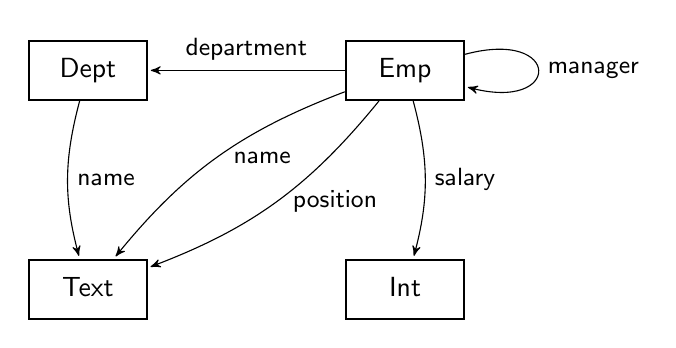
\begin{tikzpicture}
        [
            > = stealth',
            shorten > = 1pt,
            node distance = 2cm and 2.5cm,
            set/.style = {
                draw, rectangle, thick, font=\sffamily,
                minimum width=1.5cm, minimum height=.75cm,
                text height=1.5ex, text depth=.25ex},
            map/.style = {font=\small\sffamily}
        ]
        \node [set] (Dept) {Dept};
        \node [set] (Emp) [right=of Dept] {Emp};
        \node [set] (Text) [below=of Dept] {Text};
        \node [set] (Int) [below=of Emp] {Int};
        \draw [->] (Dept) to [bend right=15] node [map, right] {name} (Text);
        \draw [->] (Emp) to [bend right=15] node [map, right] {\;name} (Text);
        \draw [->] (Emp) to [bend left=15] node [map, right] {\;position} (Text);
        \draw [->] (Emp) to [bend left=15] node [map, right] {salary} (Int);
        \draw [->] (Emp) to node [map, above] {department} (Dept);
        \draw [->] (Emp) to [loop right] node [map, right] {manager} (Emp);
    \end{tikzpicture}
    \caption{Sample database schema}
\end{figure}

This model provides us with a starting point on our combinator pattern roadmap.
Any function on an entity set could be seen as a database query.  Then, all the
attributes and relationships form a set of primitive queries.  Composition of
functions becomes a binary query combinator.  With these considerations, we can
write our first composite query.

\begin{example}
    Given an employee entity, show the name of their department.
    \begin{equation*}
        \Department{.}\Name: \Emp \to \Text
    \end{equation*}
\end{example}

In this example, $\Department{.}\Name$ is a query written in Rabbit notation,
$\Emp \to \Text$ is its signature.  The period $({.})$ denotes the composition
combinator, which is a polymorphic binary operator with signature
\begin{equation*}
        (-{.}-) : (A \to B) \times (B \to C) \to (A \to C).
\end{equation*}

Even though we got a query interface, a set of primitives and one query
combinator, it doesn't yet feel like a proper query language.  Let us discuss
what is missing.

First, it is awkward that the query interface always demands an input.  It
means that we cannot express an input-free query like \emph{show a list of all
departments}.

Further, relationships between entities got a direction arbitrarily assigned to
them.  Indeed, we chose to encode the relationship between departments and
employees as a primitive with input $\Emp$ and output $\Dept$.  But this
relationship is symmetric and we may just as well be interested in finding,
\emph{for any given department, the corresponding set of employees}.  This
query cannot be encoded as a function because its signature $\Dept \to \Emp$
would incorrectly imply that there is exactly one employee per department.  The
query interface is unable to express multivalued or \emph{plural}
relationships.

The interface also fails to capture the semantics of \emph{optional} attributes
and relationships.  Such is the relationship between employees and their
managers, which, according to Figure~\ref{fig:sample-schema}, is encoded by
a primitive with signature $\Emp \to \Emp$.
But this signature implies that every employee must have a manager, which is
untrue.  Apparently, pure functional interface is too restrictive to express
the variety of relationships between database entities.

To improve this sketch of a query language, we will extend the query interface
to support optional and plural values, add primitives to express entity classes
and inverse relationships and implement common data operations in a
comprehensive library of query combinators.

This paper is organized as follows.

In Section~\ref{sec:cardinality}, we introduce query cardinality as a mo\-nadic
wrapper over its output type, which will allow us to complete our set of
primitive queries.  We also show how any database can be unfolded to the
hierarchical form.

In Section~3, we define and demonstrate how to use combinators for data
traversal, aggregation, filtering, sorting and pagination.

In Section~4, we introduce combinators for exploring hierarchical
relationships.

In Section~5, we define quotient types and show how to use them for grouping
and cube operations.

In Section~6, we show how to extend the query interface with comonadic wrapper
over its input type to support context-aware combinators.  This gives us
ability to express queries with running aggregates and parametric queries.

In Section~7, we formally describe the query interface and the composition
combinator.

In Section~8, we briefly discuss some related work.



\bibliographystyle{abbrv}
\bibliography{rbt-paper}

\end{document}

